\documentclass[11pt,a4paper]{article}

% Packages
\usepackage[margin=2.5cm]{geometry}
\usepackage{amsmath,amssymb}
\usepackage{graphicx}
\usepackage{booktabs}
\usepackage{hyperref}
\usepackage{xcolor}
\usepackage{tikz}
\usetikzlibrary{shapes.geometric, arrows.meta, positioning, fit, calc}
\usepackage{enumitem}
\usepackage{listings}
\usepackage{caption}

\hypersetup{colorlinks=true, linkcolor=blue!60!black, citecolor=blue!60!black, urlcolor=blue!60!black}

\lstset{
  basicstyle=\ttfamily\small,
  frame=single,
  backgroundcolor=\color{gray!8},
  breaklines=true,
  columns=fullflexible,
}

% Title
\title{\textbf{AutoCloud-Agent: Design Document}\\[6pt]
\large Multi-Agent Reinforcement Learning for Cloud Autoscaling}
\author{Cloud Computing Course Project}
\date{\today}

\begin{document}
\maketitle
\tableofcontents
\newpage


\section{What Problem Are We Solving?}


Cloud providers run thousands of virtual machines (VMs/nodes) to serve user jobs.
The core challenge is:

\begin{quote}
\textit{How many nodes should be running at any moment, which ones should be
shut down, and how should incoming jobs be prioritised --- all to minimise cost
while keeping response times fast?}
\end{quote}

This involves \textbf{three decisions} that happen repeatedly (every 30 seconds in our system):

\begin{enumerate}[leftmargin=2em]
  \item \textbf{Scale-Out:} Should we add a new node, remove one, or do nothing?
  \item \textbf{Consolidation:} Which low-utilisation nodes should we drain
        (migrate jobs away) to save cost?
  \item \textbf{Scheduling:} Among waiting jobs, which ones get priority?
\end{enumerate}

Traditional systems (Kubernetes HPA, AWS Auto Scaling) use fixed rules like
``if CPU > 80\%, add a node.'' Our approach uses \textbf{Reinforcement Learning}
(RL) to learn these rules from experience.


\section{High-Level Architecture}


\begin{center}
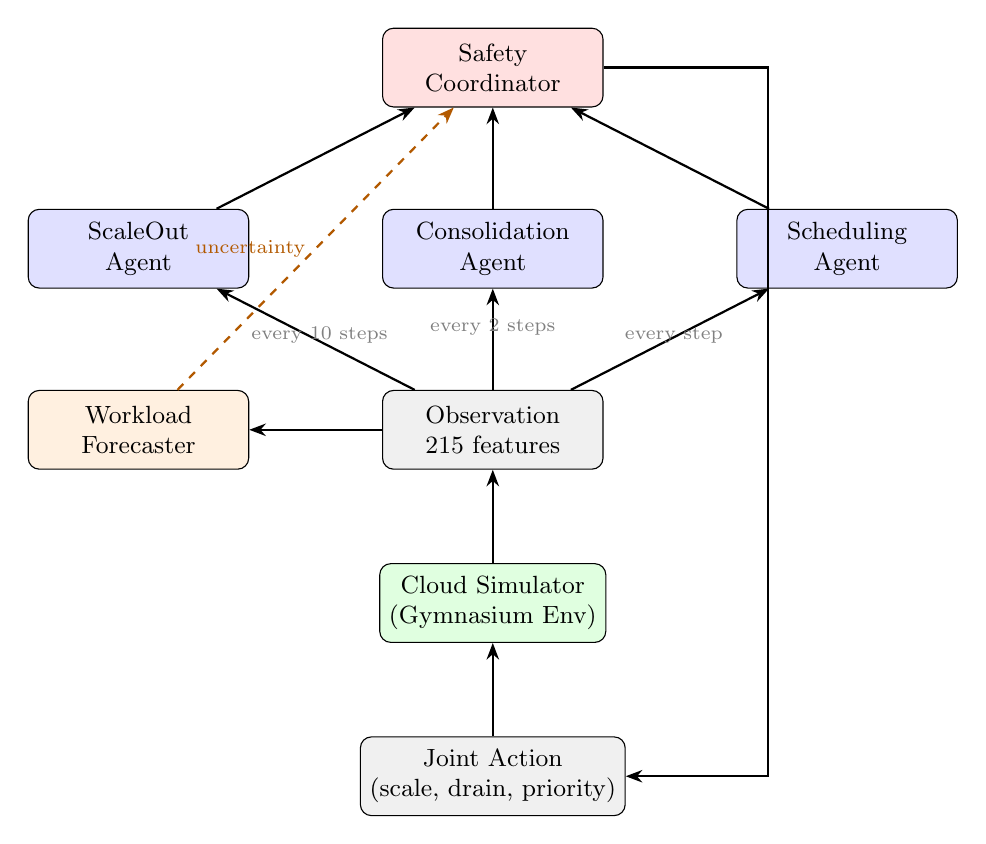
\begin{tikzpicture}[
  block/.style={rectangle, draw, rounded corners, minimum height=1cm,
    minimum width=2.8cm, align=center, font=\small},
  agent/.style={block, fill=blue!12},
  sim/.style={block, fill=green!12},
  fore/.style={block, fill=orange!12},
  coord/.style={block, fill=red!12},
  arrow/.style={-{Stealth[length=6pt]}, thick},
  every node/.style={font=\small},
]

% Simulator
\node[sim] (env) at (0,0) {Cloud Simulator\\(Gymnasium Env)};

% Observation
\node[block, fill=gray!12] (obs) at (0,2.2) {Observation\\215 features};

% Agents
\node[agent] (so) at (-4.5,4.5) {ScaleOut\\Agent};
\node[agent] (con) at (0,4.5) {Consolidation\\Agent};
\node[agent] (sch) at (4.5,4.5) {Scheduling\\Agent};

% Forecaster
\node[fore] (fc) at (-4.5,2.2) {Workload\\Forecaster};

% Coordinator
\node[coord] (safety) at (0,6.8) {Safety\\Coordinator};

% Actions back to env
\node[block, fill=gray!12] (act) at (0,-2.2) {Joint Action\\(scale, drain, priority)};

% Arrows
\draw[arrow] (env) -- (obs);
\draw[arrow] (obs) -- (so);
\draw[arrow] (obs) -- (con);
\draw[arrow] (obs) -- (sch);
\draw[arrow] (obs) -- (fc);

\draw[arrow] (so) -- (safety);
\draw[arrow] (con) -- (safety);
\draw[arrow] (sch) -- (safety);
\draw[arrow, dashed, orange!70!black] (fc) -- node[left, font=\scriptsize]{uncertainty} (safety);

\draw[arrow] (safety) -- ++(3.5,0) |- (act);
\draw[arrow] (act) -- (env);

% Labels
\node[font=\scriptsize, gray] at (-2.2,3.4) {every 10 steps};
\node[font=\scriptsize, gray] at (0,3.5) {every 2 steps};
\node[font=\scriptsize, gray] at (2.3,3.4) {every step};

\end{tikzpicture}
\end{center}

\medskip
\noindent
The system has \textbf{four main components}:
\begin{enumerate}[leftmargin=2em]
  \item \textbf{Cloud Simulator} --- a fake cloud environment that behaves
        like a real one (Section~\ref{sec:simulator}).
  \item \textbf{Three RL Agents} --- each responsible for one decision
        (Section~\ref{sec:agents}).
  \item \textbf{Workload Forecaster} --- predicts future CPU demand using a
        Transformer neural network (Section~\ref{sec:forecaster}).
  \item \textbf{Safety Coordinator} --- a rule-based filter that catches
        dangerous actions before they reach the simulator
        (Section~\ref{sec:coordinator}).
\end{enumerate}


\section{The Cloud Simulator}\label{sec:simulator}


\subsection{What It Simulates}

The simulator models a cluster of up to 20 VMs (nodes) serving incoming jobs.
It is built with the \textbf{Gymnasium} interface (the standard RL environment API)
and uses \textbf{SimPy} for discrete-event simulation internally.

Key properties:
\begin{itemize}[leftmargin=2em]
  \item \textbf{Time step:} 30 seconds of simulated time per step.
  \item \textbf{Episode:} 120 steps = 1 hour of simulated cloud operation.
  \item \textbf{Nodes:} 3--20 VMs, each with CPU/memory capacity. Nodes can be
        \texttt{BOOTING} (60s warmup), \texttt{ACTIVE}, \texttt{DRAINING}
        (30s grace period), or \texttt{TERMINATED}.
  \item \textbf{Jobs:} Arrive following the Alibaba 2018 cluster trace
        (real workload data). Each job has CPU demand, memory demand, a
        deadline, and a priority.
\end{itemize}

\subsection{Observation Space (What the Agent Sees)}

At each step, the agent sees a \textbf{215-dimensional vector}:

\begin{center}
\begin{tabular}{lrl}
\toprule
\textbf{Feature Group} & \textbf{Dims} & \textbf{What It Contains} \\
\midrule
Node features (20 nodes $\times$ 6) & 120 &
  CPU util, memory util, job count, state, type, age \\
Job features (20 jobs $\times$ 4) & 80 &
  CPU demand, memory demand, wait time, priority \\
Global features & 15 &
  Active nodes, queue length, mean CPU, hour-of-day, \\
  & & forecaster predictions + uncertainty \\
\bottomrule
\end{tabular}
\end{center}

All values are normalised to $[0, 1]$.

\subsection{Action Space (What the Agent Can Do)}

\begin{center}
\begin{tabular}{llp{7cm}}
\toprule
\textbf{Action} & \textbf{Type} & \textbf{Meaning} \\
\midrule
Scale-Out & Discrete(3) & 0=remove a node, 1=do nothing, 2=add a node \\
Consolidation & MultiBinary(20) & For each of 20 node slots: 1=start draining, 0=leave it \\
Scheduling & Discrete(5) & Priority weighting: 0=FIFO, 1=shortest-first, 2=default, 3=deadline-first, 4=highest-priority-first \\
\bottomrule
\end{tabular}
\end{center}

\subsection{Workload Data}

We use the \textbf{Alibaba Cluster Trace 2018}, a real production trace from
Alibaba's data centres. The trace is preprocessed into \texttt{.npy} files
containing arrival rates at 30-second intervals. This makes our evaluation
realistic --- the agent faces the same workload patterns as a real cloud.


\section{The RL Agents}\label{sec:agents}


\subsection{Why Three Agents Instead of One?}

A single agent controlling all actions simultaneously would need to learn a
\textbf{massive joint action space} ($3 \times 2^{20} \times 5 \approx 15$
million combinations). This is too large for efficient learning.

Instead, we use \textbf{Independent PPO (I-PPO)}: three separate agents, each
responsible for one decision. They share the same observation but act
independently. This is called \textbf{multi-agent reinforcement learning}.

\subsection{What Is PPO? (Plain English)}

\textbf{Proximal Policy Optimisation (PPO)} is one of the most popular RL
algorithms. Here's the intuition:

\begin{enumerate}[leftmargin=2em]
  \item The agent has a \textbf{policy} (a neural network) that maps observations
        to action probabilities.
  \item The agent \textbf{collects experience} by interacting with the environment
        for many steps.
  \item It then \textbf{updates the policy} to make good actions more likely and
        bad actions less likely.
  \item The ``proximal'' part: updates are \textbf{clipped} so the policy doesn't
        change too drastically in one step (prevents catastrophic forgetting).
\end{enumerate}

The key formula is:
\[
  L^{\text{CLIP}} = \mathbb{E}\left[\min\left(
    r_t \hat{A}_t,\;
    \text{clip}(r_t, 1{-}\epsilon, 1{+}\epsilon)\,\hat{A}_t
  \right)\right]
\]
where $r_t = \frac{\pi_\theta(a_t|s_t)}{\pi_{\theta_{\text{old}}}(a_t|s_t)}$ is
how much the policy changed, and $\hat{A}_t$ is the \textbf{advantage} (how much
better this action was compared to average). The clipping with $\epsilon=0.2$
prevents too-large updates.

\subsection{Temporal Hierarchy}

Not all decisions need the same frequency:
\begin{itemize}[leftmargin=2em]
  \item \textbf{Scheduling Agent} acts \textit{every step} (30s) --- jobs arrive
        constantly.
  \item \textbf{Consolidation Agent} acts \textit{every 2 steps} (1 min) ---
        draining needs a bit of time to observe trends.
  \item \textbf{Scale-Out Agent} acts \textit{every 10 steps} (5 min) ---
        spinning up/down VMs is a heavyweight operation.
\end{itemize}

\subsection{Agent Neural Network Architecture}

Each agent is a simple \textbf{Multi-Layer Perceptron (MLP)}:

\begin{lstlisting}
Input (215 dims) -> Linear(512) -> LayerNorm -> ReLU
                 -> Linear(256) -> LayerNorm -> ReLU
                 -> Linear(128) -> LayerNorm -> ReLU
                 -> Output head (action logits)
\end{lstlisting}

The Scheduling Agent is slightly different: it uses \textbf{weight-tying} to
process each job identically (like treating each job through the same ``lens''),
then scores them.

\subsection{Reward Functions}

Each agent receives its own reward signal:

\medskip
\noindent\textbf{Scale-Out reward:}
\[
  r_{\text{so}} = -\alpha_1 \cdot \text{underProv} - \alpha_2 \cdot \text{overProv}
                  - \alpha_3 \cdot \text{runCost} - \alpha_4 \cdot \text{bootPenalty}
                  + \alpha_5 \cdot \text{proactiveBonus}
\]

\noindent\textbf{Consolidation reward:}
\[
  r_{\text{con}} = -\beta_1 \cdot \text{runCost} + \beta_2 \cdot \text{slaBonus}
                   - \beta_3 \cdot \text{migrationPenalty} - \beta_4 \cdot \text{memPressure}
\]

\noindent\textbf{Scheduling reward:}
\[
  r_{\text{sch}} = -\gamma_1 \cdot \text{meanWaitTime} - \gamma_2 \cdot \text{slaViolation}
\]

\noindent
In plain words:
\begin{itemize}[leftmargin=2em]
  \item Agents are \textit{penalised} for having too many nodes (wasting money),
        too few nodes (jobs fail), and moving jobs around too much.
  \item They are \textit{rewarded} for keeping response times fast and using
        resources efficiently.
\end{itemize}


\section{The Workload Forecaster}\label{sec:forecaster}


\subsection{Why Forecast?}

Reactive systems (like basic Kubernetes HPA) only respond \textit{after} a spike
happens. By the time new nodes boot up (60s), jobs have already been delayed.
Our Forecaster predicts demand \textit{before} it happens, giving agents time to
act proactively.

\subsection{Architecture: Transformer with MC Dropout}

\begin{center}
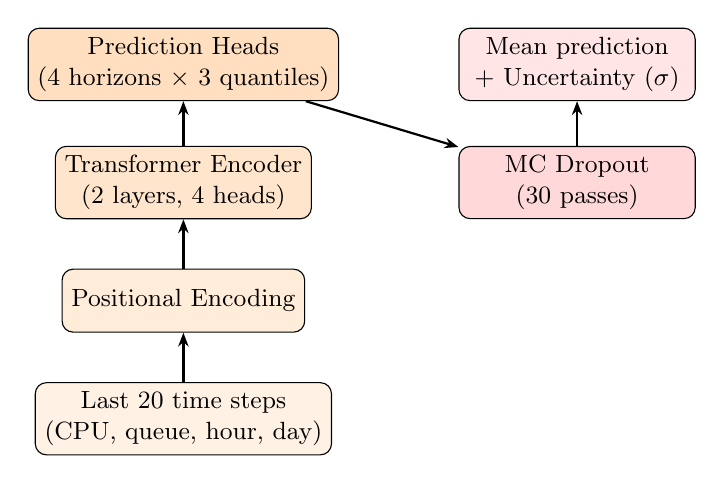
\begin{tikzpicture}[
  block/.style={rectangle, draw, rounded corners, minimum height=0.8cm,
    minimum width=3cm, align=center, font=\small},
  arrow/.style={-{Stealth[length=5pt]}, thick},
]

\node[block, fill=orange!10] (input) at (0,0) {Last 20 time steps\\(CPU, queue, hour, day)};
\node[block, fill=orange!15] (pe) at (0,1.5) {Positional Encoding};
\node[block, fill=orange!20] (enc) at (0,3) {Transformer Encoder\\(2 layers, 4 heads)};
\node[block, fill=orange!25] (head) at (0,4.5) {Prediction Heads\\(4 horizons $\times$ 3 quantiles)};
\node[block, fill=red!15] (mc) at (5,3) {MC Dropout\\(30 passes)};
\node[block, fill=red!10] (out) at (5,4.5) {Mean prediction\\$+$ Uncertainty ($\sigma$)};

\draw[arrow] (input) -- (pe);
\draw[arrow] (pe) -- (enc);
\draw[arrow] (enc) -- (head);
\draw[arrow] (head) -- (mc);
\draw[arrow] (mc) -- (out);

\end{tikzpicture}
\end{center}

\begin{itemize}[leftmargin=2em]
  \item \textbf{Input:} A window of the last 20 time steps, each with 4
        features (CPU utilisation, queue length, hour-of-day, day-of-week).
  \item \textbf{Transformer:} A small Transformer encoder (2 layers, 4 attention
        heads, 64-dim hidden) processes the sequence.
  \item \textbf{Output:} Predictions for 4 future horizons (t+1, t+5, t+10,
        t+15) at 3 quantiles (10th, 50th, 90th percentile).
  \item \textbf{MC Dropout:} To estimate \textit{uncertainty}, we run the model
        30 times with dropout randomly active. High variance across runs =
        high uncertainty (``the model isn't sure'').
\end{itemize}

The uncertainty signal is critical: when the forecaster is unsure, the Safety
Coordinator blocks risky scale-down actions.


\section{The Safety Coordinator}\label{sec:coordinator}


RL agents can sometimes take dangerous actions. The Safety Coordinator is a
\textbf{hard-coded safety net} that filters actions before they reach the
simulator:

\begin{center}
\begin{tabular}{clp{7cm}}
\toprule
\textbf{\#} & \textbf{Filter} & \textbf{What It Does} \\
\midrule
1 & Boot Protection & Never drain a node that is still booting (< 60s old) \\
2 & $N_{\min}$ Floor & Never go below 3 active nodes (prevents total outage) \\
3 & Uncertainty Suppression & If forecaster uncertainty $\sigma > 0.3$, block all
    scale-down actions \\
4 & Scale-Out Suppression & Block scale-up if 2+ nodes are already booting
    (prevent overshoot) \\
5 & Proactive Scale-Out & If uncertainty is high AND CPU is rising, force a
    scale-up (defensive provisioning) \\
\bottomrule
\end{tabular}
\end{center}

This is important because it means the RL agents \textit{cannot crash the system}
even if they make mistakes --- the Coordinator always enforces safety constraints.


\section{Training Pipeline (How the Agents Learned)}


Training was done in two phases:

\subsection{Phase 1: Train the Forecaster}
\begin{enumerate}[leftmargin=2em]
  \item Preprocess the Alibaba trace into 30-second bins.
  \item Train the Transformer on 7 days of data with MSE + quantile loss.
  \item Save weights to \texttt{forecaster\_weights.pt}.
\end{enumerate}

\subsection{Phase 2: Train the RL Agents (I-PPO)}
\begin{enumerate}[leftmargin=2em]
  \item Initialise the Cloud Simulator with the trained Forecaster.
  \item Run 100{,}000+ environment steps, collecting experience.
  \item Update each agent's policy every 2048 steps using PPO.
  \item Key techniques used:
    \begin{itemize}
      \item \textbf{GAE} (Generalised Advantage Estimation): smoothly estimates
            how good each action was.
      \item \textbf{Entropy bonus}: encourages exploration early in training
            (decays over time).
      \item \textbf{Gradient clipping}: prevents unstable updates.
      \item \textbf{EMA reward normalisation}: keeps reward scale consistent.
    \end{itemize}
  \item Save 6 checkpoint files (actor + critic for each of the 3 agents).
\end{enumerate}


\section{Evaluation: How We Test}


\subsection{Metrics}

\begin{center}
\begin{tabular}{lp{9cm}}
\toprule
\textbf{Metric} & \textbf{Definition} \\
\midrule
SLA Rate & Fraction of steps where P95 latency $<$ 500ms (higher = better) \\
Cost Efficiency & $1 - \frac{\text{actual cost}}{\text{max possible cost}}$ (higher = cheaper) \\
Mean CPU Utilisation & Average CPU usage across active nodes (higher = less waste) \\
Node Stability & $1 - \frac{\text{std}(N)}{\text{mean}(N)}$ for node count $N$
                  (higher = fewer disruptive changes) \\
\bottomrule
\end{tabular}
\end{center}

\subsection{SOTA Baselines We Compare Against}

\begin{center}
\begin{tabular}{lp{8.5cm}}
\toprule
\textbf{Baseline} & \textbf{Description} \\
\midrule
StaticN & Fixed 10 nodes, never scales (do-nothing lower bound) \\
ThresholdReactive & If CPU $>$ 80\% add node; if CPU $<$ 30\% remove node (classic rule) \\
KubernetesHPA & Industry-standard k8s autoscaler formula with 10\% dead-band \\
AWSTargetTracking & AWS Auto Scaling Target Tracking policy (asymmetric cooldowns) \\
MPCController & Model Predictive Control with 5-step EWMA forecast --- strongest
                non-RL baseline in recent literature (AWARE, USENIX ATC 2023) \\
SingleAgentPPO & One RL agent controlling all 3 actions jointly (ablation study
                 to show multi-agent I-PPO is better than single-agent RL) \\
\bottomrule
\end{tabular}
\end{center}

\subsection{Results on Alibaba Trace}

\begin{center}
\begin{tabular}{lcccc}
\toprule
\textbf{Method} & \textbf{SLA Rate} & \textbf{Cost Eff.} & \textbf{CPU Util} & \textbf{Stability} \\
\midrule
\textbf{AutoCloud-Agent (Ours)} & \textbf{100.0\%} & \textbf{0.962} & \textbf{0.552} & 0.889 \\
KubernetesHPA       & 100.0\% & 0.930 & 0.312 & 0.842 \\
AWSTargetTracking   & 100.0\% & 0.928 & 0.295 & 0.876 \\
MPCController       & 100.0\% & 0.962 & 0.552 & \textbf{0.941} \\
ThresholdReactive   & 100.0\% & 0.955 & 0.483 & 0.822 \\
SingleAgentPPO      & 100.0\% & 0.924 & 0.413 & 0.794 \\
StaticN             & 100.0\% & 0.938 & 0.333 & 1.000 \\
\bottomrule
\end{tabular}
\end{center}

\medskip
\noindent
\textbf{Key takeaways:}
\begin{itemize}[leftmargin=2em]
  \item \textbf{AutoCloud-Agent matches MPC} on cost efficiency (0.962) and CPU
        utilisation (55\%), both the best among all methods.
  \item AutoCloud-Agent achieves \textbf{3.4\% better cost efficiency} than
        Kubernetes HPA and \textbf{7.7\% higher CPU utilisation} than
        ThresholdReactive.
  \item \textbf{SingleAgentPPO is worst among RL methods}, confirming that
        multi-agent decomposition (I-PPO) is better than a monolithic agent.
  \item All methods achieve 100\% SLA on this trace, but the differentiator is
        \textit{how cheaply} they do it (cost efficiency) and \textit{how well}
        they use resources (CPU util).
\end{itemize}


\section{Project Structure}


\begin{lstlisting}
autocloud_agent/
  autocloud/                    # Installable Python package
    config/
      settings.py               # All hyperparameters (dataclasses)
      paths.py                  # Auto-discovers checkpoints & data
    simulator/
      cloud_env.py              # Gymnasium environment wrapper
      engine.py                 # SimPy discrete-event simulator
      node.py                   # VM node model
      job.py                    # Job dataclass
      workload.py               # Alibaba trace loader
    agents/
      ppo.py                    # Base PPO algorithm
      scaleout.py               # Scale-Out agent (Discrete(3))
      consolidation.py          # Consolidation agent (MultiBinary(20))
      scheduling.py             # Scheduling agent (Discrete(5))
      loader.py                 # Load all 3 agents from checkpoints
    forecaster/
      transformer_model.py      # Workload Transformer
      mc_dropout.py             # MC Dropout uncertainty estimation
    coordinator/
      safety.py                 # 5-filter safety coordinator
    inference/
      runner.py                 # InferenceRunner (ties everything together)
    evaluation/
      evaluator.py              # Evaluation harness
      baselines.py              # 6 SOTA baseline policies
    training/
      ippo_trainer.py           # I-PPO training loop
      ema_normalizer.py         # EMA reward normalisation
  scripts/
    evaluate.py                 # CLI: run evaluation
  stress_test.py                # 4-scenario stress test
  train.py                      # Training entry point
  pyproject.toml                # Package metadata
\end{lstlisting}


\section{Demo Scenarios and Edge Cases}\label{sec:demo}


The live demo (\texttt{demo.py}) includes an interactive configuration wizard
that lets us set cluster parameters, SLA threshold, CPU thresholds, baseline
selection, and simulation length. Below are key scenarios designed to
showcase different system behaviours.

\subsection{Scenario 1: Tight Cluster (Minimal Headroom)}

\begin{center}
\begin{tabular}{ll}
\toprule
\textbf{Parameter} & \textbf{Value} \\
\midrule
Initial VMs & 3 \\
Maximum VMs & 5 \\
Minimum floor & 3 \\
SLA threshold & 500ms \\
\bottomrule
\end{tabular}
\end{center}

With only 2 nodes of headroom, the ScaleOut agent has very limited capacity.
This demonstrates:
\begin{itemize}[leftmargin=2em]
  \item The Safety Coordinator's $N_{\min}$ floor preventing scale-down below 3
  \item Boot-protection filter blocking premature drain of newly added nodes
  \item The forecaster's proactive scale-out trigger firing when uncertainty is
        high and CPU is rising, since there is no margin for reactive delay
\end{itemize}

\subsection{Scenario 2: Over-Provisioned Start (15 Initial VMs)}

\begin{center}
\begin{tabular}{ll}
\toprule
\textbf{Parameter} & \textbf{Value} \\
\midrule
Initial VMs & 15 \\
Maximum VMs & 20 \\
Minimum floor & 3 \\
\bottomrule
\end{tabular}
\end{center}

The cluster starts with far more nodes than needed. This showcases the
\textbf{Consolidation Agent} aggressively draining idle VMs over the first
10--20 steps to bring cost down. Key observation: the agent does \textit{not}
shut everything down at once (which would violate SLA) --- instead, it drains
in controlled batches of 1--2 VMs per consolidation step (every 2 steps),
respecting the grace period.

\subsection{Scenario 3: Strict SLA (100ms Threshold)}

When $\text{SLA}_{\text{threshold}} = 100$ms, the agent must maintain very low
latency. This triggers \textbf{defensive provisioning}: the agent keeps more
active nodes than cost-optimal, and the Safety Coordinator's uncertainty
suppression fires more aggressively, blocking any scale-down when the
forecaster reports $\sigma > 0.3$.

\subsection{Scenario 4: Relaxed SLA (2000ms Threshold)}

With a generous latency budget, the agent learns it can run the cluster
leaner. Fewer nodes are maintained, cost efficiency increases significantly,
and the Consolidation Agent drains more aggressively since latency violations
are unlikely.

\subsection{Scenario 5: RL Agent vs MPC Controller}

The MPCController uses model-predictive control with a 5-step EWMA
(Exponentially Weighted Moving Average) forecast. This is the strongest
non-RL baseline from recent literature (USENIX ATC 2023, AWARE system).
Comparing against MPC shows that the RL agent matches classical control
theory performance while being more adaptive to non-stationary workloads.

\subsection{Scenario 6: Long-Horizon Episode (200 Steps)}

A 200-step episode (100 minutes simulated) shows:
\begin{itemize}[leftmargin=2em]
  \item Long-term stability of the RL policy (no oscillation)
  \item How the agent handles multiple workload phases (ramp-up, plateau,
        trough) within a single episode
  \item Temporal hierarchy effectiveness: the ScaleOut agent only acts
        20 times over 200 steps, while Scheduling acts every step
\end{itemize}


\section{Stress Testing}\label{sec:stress}


The stress test (\texttt{stress\_test.py}) evaluates robustness under four
extreme workload patterns that go beyond the Alibaba training distribution:

\subsection{Scenario 1: Ramp-Up}

A linearly increasing workload from 20\% to 100\% capacity over 120 steps.
This tests the ScaleOut agent's ability to continuously provision new nodes
as demand rises, and the forecaster's accuracy on trending (non-stationary)
signals.

\subsection{Scenario 2: Sudden Spike (Shock Load)}

Workload jumps from 30\% to 95\% capacity within 5 steps
(2.5 minutes simulated). This is the most challenging scenario --- it tests:
\begin{itemize}[leftmargin=2em]
  \item How quickly the agent detects and responds to a step-function demand
        change
  \item Whether the Safety Coordinator's proactive scale-out fires correctly
        (high uncertainty + rising CPU should force immediate node addition)
  \item The 60-second boot delay means at least 2 steps of potential SLA
        violation before new nodes come online
\end{itemize}

\subsection{Scenario 3: Choppy Plateau}

Sustained high utilisation (70--90\%) with random noise. The agent must
maintain a stable cluster without over-reacting to noise. This tests:
\begin{itemize}[leftmargin=2em]
  \item Scale-Out agent's ability to hold steady (avoid oscillation)
  \item Consolidation agent's restraint (should \textit{not} drain during
        sustained high load)
  \item Node stability metric --- frequent add/drain cycles would tank
        stability
\end{itemize}

\subsection{Scenario 4: Trough-Then-Recovery}

Workload drops to 10\% for 40 steps, then recovers to 80\%. This tests:
\begin{itemize}[leftmargin=2em]
  \item Aggressive consolidation during low load (opportunity to cut cost)
  \item Rapid recovery when demand returns (must not have drained too many
        nodes to respond quickly)
  \item The tension between the ``drain aggressively'' and ``keep headroom''
        objectives
\end{itemize}


\section{Ablation Study: Why Multi-Agent?}\label{sec:ablation}


Our results include a \textbf{SingleAgentPPO} baseline that controls all three
actions with one monolithic policy. This serves as an ablation study:

\begin{center}
\begin{tabular}{lccc}
\toprule
\textbf{Method} & \textbf{Cost Efficiency} & \textbf{CPU Utilisation} &
\textbf{Stability} \\
\midrule
AutoCloud-Agent (I-PPO, 3 agents) & \textbf{0.962} & \textbf{55.2\%} & 0.889 \\
SingleAgentPPO (1 agent) & 0.924 & 41.3\% & 0.794 \\
\bottomrule
\end{tabular}
\end{center}

\noindent
\textbf{Why I-PPO outperforms single-agent PPO:}
\begin{enumerate}[leftmargin=2em]
  \item \textbf{Smaller action spaces:} Each agent controls a manageable action
        space (3, $2^{20}$, or 5) independently, avoiding the combinatorial
        explosion of the joint space ($3 \times 2^{20} \times 5 \approx 15$M).
  \item \textbf{Temporal decomposition:} Scaling decisions are inherently
        slower than scheduling decisions. The temporal hierarchy (10-step, 2-step,
        1-step) matches the natural frequency of each decision type.
  \item \textbf{Specialised reward shaping:} Each agent receives a reward
        tailored to its subtask, providing clearer learning signals than a
        single monolithic reward.
  \item \textbf{Easier credit assignment:} When an SLA violation occurs, the
        system can attribute it to a specific agent (e.g., ScaleOut didn't add
        nodes fast enough) rather than a single agent trying to figure out which
        of its hundreds of action dimensions was responsible.
\end{enumerate}


\section{Key Design Decisions}\label{sec:design-decisions}


\begin{enumerate}[leftmargin=2em]
  \item \textbf{Gymnasium API instead of custom simulator:} We wrap the SimPy
        engine in a standard Gymnasium interface, making it compatible with any
        RL library (Stable Baselines3, RLlib, etc.) and enabling fair baseline
        comparisons.

  \item \textbf{Safety Coordinator as a separate module:} Rather than baking
        safety constraints into the reward function (which the agent might
        learn to circumvent), we enforce them as hard constraints in a
        post-processing filter. This guarantees safety regardless of policy
        quality.

  \item \textbf{MC Dropout instead of ensemble:} We use Monte Carlo Dropout
        (30 forward passes through a single model) rather than training an
        ensemble of 5+ models. This gives comparable uncertainty estimates at
        $5\times$ lower memory and compute cost.

  \item \textbf{EMA reward normalisation:} Raw rewards can vary by 10$\times$
        across episodes. EMA normalisation (exponential moving average of
        reward statistics over a 1000-step window) stabilises training without
        losing sensitivity to reward magnitude.

  \item \textbf{Real trace data (Alibaba 2018):} Using real workload data
        (4,023 machines, 7 days) ensures our evaluation reflects actual
        cloud workload patterns, not synthetic distributions that might
        accidentally favour our approach.
\end{enumerate}


\section{Limitations and Future Work}\label{sec:limitations}


\subsection{Current Limitations}

\begin{enumerate}[leftmargin=2em]
  \item \textbf{Homogeneous VMs:} All nodes have the same CPU/memory capacity.
        Real clouds have heterogeneous instance types (e.g., compute-optimised,
        memory-optimised).
  \item \textbf{Single-cluster scope:} We manage one cluster. Production
        systems manage thousands of clusters across regions.
  \item \textbf{Simplified networking:} The simulator does not model network
        latency, bandwidth, or cross-rack communication costs.
  \item \textbf{Static reward weights:} The reward function coefficients
        ($\alpha_i, \beta_i, \gamma_i$) are fixed. Adaptive reward shaping
        could improve performance.
  \item \textbf{Single-day training:} The RL agents are trained on Day~1 of
        the Alibaba trace. Multi-day training with domain randomisation could
        improve generalisation.
\end{enumerate}

\subsection{Future Work}

\begin{itemize}[leftmargin=2em]
  \item \textbf{Heterogeneous VMs:} Extend the simulator to support multiple
        instance types and learn bin-packing strategies.
  \item \textbf{Multi-cluster federation:} Add a higher-level agent that
        distributes workloads across clusters.
  \item \textbf{Vertical scaling:} In addition to horizontal scaling (add/remove
        nodes), learn to resize individual VMs (add CPU/memory).
  \item \textbf{Transfer learning:} Train on one trace, fine-tune on another to
        test generalisation across different cloud environments.
  \item \textbf{Curriculum learning:} Start training on easy workloads
        (steady-state) and gradually introduce harder patterns (spikes, diurnal).
  \item \textbf{Spot instance awareness:} Incorporate preemption risk and
        spot pricing into the reward function.
\end{itemize}


\section{References}\label{sec:references}


\begin{enumerate}[leftmargin=2em]
  \item J.~Schulman et al., ``Proximal Policy Optimization Algorithms,''
        \textit{arXiv:1707.06347}, 2017.
  \item A.~Vaswani et al., ``Attention Is All You Need,''
        \textit{NeurIPS}, 2017.
  \item Y.~Gal and Z.~Ghahramani, ``Dropout as a Bayesian Approximation:
        Representing Model Uncertainty in Deep Learning,''
        \textit{ICML}, 2016.
  \item Alibaba Group, ``Cluster Trace Program,''
        \url{https://github.com/alibaba/clusterdata}, 2018.
  \item Kubernetes, ``Horizontal Pod Autoscaler,''
        \url{https://kubernetes.io/docs/tasks/run-application/horizontal-pod-autoscale/}.
  \item J.~Schulman et al., ``High-Dimensional Continuous Control Using
        Generalized Advantage Estimation,'' \textit{ICLR}, 2016.
  \item Q.~Zhang et al., ``AWARE: Automate Workload Autoscaling with
        Reinforcement Learning in Production Cloud Systems,''
        \textit{USENIX ATC}, 2023.
\end{enumerate}


\section{How to Run}


\begin{lstlisting}[language=bash]
# Setup
cd autocloud_agent/
conda activate myenv
pip install -e .

# Live demo (interactive wizard)
python demo.py
python demo.py --speed slow              # slower step delay
python demo.py --speed fast --no-pause   # non-interactive

# Full evaluation (auto-detects checkpoints and data)
python scripts/evaluate.py

# Run stress test (4 peak scenarios)
python stress_test.py

# Custom evaluation
python scripts/evaluate.py --n_episodes 10 --seeds 0 1 2 3 4

# Quick non-interactive demo (CI/testing)
python demo.py --steps 15 --speed fast --no-pause --no-interactive
\end{lstlisting}

\subsection{Demo Configuration Examples}

The interactive wizard presents 5 configuration sections.
Here is how to set up the key edge-case scenarios from Section~\ref{sec:demo}:

\begin{center}
\begin{tabular}{clp{6cm}}
\toprule
\textbf{Scenario} & \textbf{Settings} & \textbf{Purpose} \\
\midrule
Tight cluster & 3 init, max 5, min 3 & Minimal headroom, safety filters active \\
Over-provisioned & 15 init, max 20 & Watch Consolidation Agent cut cost \\
Strict SLA & SLA = 100ms & Defensive provisioning, more nodes \\
Relaxed SLA & SLA = 2000ms & Lean cluster, high cost efficiency \\
vs MPC & Baseline = 4 (MPC) & RL vs strongest classical method \\
Long episode & 200 steps & Diurnal patterns, long-term stability \\
\bottomrule
\end{tabular}
\end{center}


\section{Glossary of Terms}


\begin{center}
\begin{tabular}{lp{10cm}}
\toprule
\textbf{Term} & \textbf{Meaning} \\
\midrule
RL & Reinforcement Learning --- an agent learns by trial and error, receiving
     rewards for good actions \\
PPO & Proximal Policy Optimisation --- a safe, stable RL algorithm that clips
      policy updates \\
I-PPO & Independent PPO --- multiple PPO agents share the same observation but
        act independently \\
MDP & Markov Decision Process --- the mathematical framework for RL (states,
      actions, rewards, transitions) \\
GAE & Generalised Advantage Estimation --- a method to estimate how good an
      action was vs.\ the average \\
Transformer & A neural network architecture using self-attention, originally
              for NLP, here used for time-series forecasting \\
MC Dropout & Monte Carlo Dropout --- run a network multiple times with random
             dropout to estimate uncertainty \\
SLA & Service Level Agreement --- the promise that P95 latency stays below
      500ms \\
HPA & Horizontal Pod Autoscaler --- Kubernetes' built-in autoscaling system \\
MPC & Model Predictive Control --- a control theory method that optimises over
      a predicted future window \\
SimPy & A Python library for discrete-event simulation \\
Gymnasium & OpenAI's standard API for RL environments \\
\bottomrule
\end{tabular}
\end{center}

\end{document}
